% Harus dimuat terlebih dahulu, digunakan agar file PDF memiliki format karakter yang benar.
% Untuk informasi lebih lanjut, lihat https://ctan.org/pkg/cmap.
\RequirePackage{cmap}

% Format dokumen sebagai paper konferensi menggunakan aturan IEEEtran terbaru (v1.8b).
% Untuk informasi lebih lanjut, lihat http://www.michaelshell.org/tex/ieeetran/.
\documentclass[conference]{IEEEtran}[2015/08/26]

% Format encoding font dan input menjadi 8-bit UTF-8.
\usepackage[T1]{fontenc}
\usepackage[utf8]{inputenc}

% Format bahasa menjadi bahasa german dan inggris.
\usepackage[indonesian]{babel}

% Digunakan untuk tujuan demonstrasi.
\usepackage{mwe}

% Digunakan untuk menampilkan font dengan style yang lebih baik.
\usepackage[zerostyle=b,scaled=.75]{newtxtt}

% Digunakan untuk menampilkan tabel dengan style yang lebih baik.
\usepackage{booktabs}

% Digunakan untuk menampilkan gambar pada dokumen.
\usepackage{graphicx}

% Digunakan untuk menampilkan potongan kode.
\usepackage{listings}
\lstset{
  basicstyle=\ttfamily,
  columns=fixed,
  basewidth=.5em,
  xleftmargin=0.5cm,
  captionpos=b
}

% Digunakan agar backticks (`) dapat dirender pada PDF.
% Untuk informasi lebih lanjut, lihat https://tex.stackexchange.com/a/341057/9075.
\usepackage{upquote}

% Digunakan untuk menyeimbangkan bagian akhir dokumen dengan dua kolom.
\usepackage{balance}

% Digunakan untuk menampilkan pustaka.
\usepackage[square,comma,numbers,sort&compress]{natbib}

% Mengubah format ukuran teks pada natbib.
\renewcommand{\bibfont}{\normalfont\footnotesize}

% Menambah nama penulis ketika menggunakan perintah \citet.
% Untuk informasi lebih lanjut, lihat https://tex.stackexchange.com/a/76075/9075.
\usepackage{etoolbox}
\makeatletter
\patchcmd{\NAT@test}{\else \NAT@nm}{\else \NAT@hyper@{\NAT@nm}}{}{}
\makeatother

% Digunakan untuk melakukan linewrap pada pustaka dengan url yang panjang
% jika terdapat hyphens
\usepackage[hyphens]{url}

% Digunakan untuk menambah hyperlink pada referensi.
\usepackage{hyperref}

% Menonaktifkan warna dan bookmark pada hyperref.
\hypersetup{hidelinks,
  colorlinks=true,
  allcolors=black,
  pdfstartview=Fit,
  breaklinks=true
}

% Digunakan untuk membenarkan hyperref pada gambar.
\usepackage[all]{hypcap}

% Digunakan untuk menampilkan beberapa gambar
\usepackage[caption=false,font=footnotesize]{subfig}

\usepackage{stfloats}

% Tambahkan format tanda hubung yang benar di sini
\hyphenation{
  ro-ket
  me-ngem-bang-kan
  per-hi-tu-ngan
}

\usepackage{enumitem}
\setlist{parsep=0pt,listparindent=\parindent}

\begin{document}

  % Ubah kalimat berikut sesuai dengan judul penelitian.
\title{Prediksi Jumlah Kalori yang Terbakar saat Berolahraga dengan Treadmill Berbasis Kamera Menggunakan \emph{Convolutional Neural Network}}

% Ubah kalimat-kalimat berikut sesuai dengan nama, institusi, alamat dan kontak penulis.
\author{
  \IEEEauthorblockN{Dimas Aditya Maulana Fajri}
  \IEEEauthorblockA{\textit{Dept. Teknik Komputer}\\
  \textit{Institut Teknologi Sepuluh Nopember}\\
    Surabaya, Indonesia 60111\\
    dimas.adityamf@gmail.com}
  \and
  \IEEEauthorblockN{Eko Mulyanto Yuniarno}
  \IEEEauthorblockA{\textit{Dept. Teknik Komputer}\\
  \textit{Institut Teknologi Sepuluh Nopember}\\
    Surabaya, Indonesia 60111\\
    ekomulyanto@ee.its.ac.id}
  \and
  \IEEEauthorblockN{Arief Kurniawan}
  \IEEEauthorblockA{\textit{Dept. Teknik Komputer}\\
  \textit{Institut Teknologi Sepuluh Nopember}\\
    Surabaya, Indonesia 60111\\
    arifku@ee.its.ac.id} 
}

% Digunakan untuk menampilkan judul dan deskripsi penulis.
\maketitle

% Fakultas Teknologi Elektrodan Informatika Cerdas\\
%     Institut Teknologi Sepuluh Nopember\\
%     Surabaya, Indonesia 60111\\
%     dimas.adityamf@gmail.com}
  % Mengubah keterangan `Abstract` ke bahasa indonesia.
% Hapus bagian ini untuk mengembalikan ke format awal.
\renewcommand\abstractname{Abstrak}

\begin{abstract}

  % Ubah paragraf berikut sesuai dengan abstrak dari penelitian.
  Obesitas merupakan keadaan dimana terdapat penumpukan lemak pada tubuh seseorang yang menyebabkan berat badan berada pada nilai di atas normal. Ketidak seimbangan kalori yang dikonsumsi dan yang digunakan menyebabkan kelebihan berat badan. Salah satu aktivitas yang bisa mengurangi kelebihan berat badan adalah dengan olahraga yang memiliki kualitas aktivitas yang baik. Olahraga pada treadmill merupakan salah satu aktivitas yang dapat dilakukan dan melakukan pengukuran kalori yang terbakar. Namun perhitungan kalori pada treadmill masih belum akurat dan praktis. Penelitian ini membuat sistem yang dapat memprediksi kalori yang terbakar saat olahraga pada treadmill menggunakan citra video dengan kamera. Metode yang digunakan dengan melakukan pengambilan data yang kemudian dideteksi pose untuk postur tubuh. Model dibuat menggunakan CNN. Hasil deteksi berupa banyak langkah dan waktu untuk dilakukan prediksi kalori. Prediksi menggunakan regresi linear dan perhitungan MET. Hasil akhir yang diharapkan dapat memprediksi jumlah kalori yang terbakar dari citra video.

\end{abstract}

% Mengubah keterangan `Index terms` ke bahasa indonesia.
% Hapus bagian ini untuk mengembalikan ke format awal.
\renewcommand\IEEEkeywordsname{Kata kunci}

\begin{IEEEkeywords}

  % Ubah kata-kata berikut sesuai dengan kata kunci dari penelitian.
  Obesitas; kalori, prediksi, video.

\end{IEEEkeywords}


  % Ubah bagian berikut sesuai dengan konten-konten yang akan dimasukkan pada dokumen
  % Ubah judul dan label berikut sesuai dengan yang diinginkan.
\section{Pendahuluan}
\label{sec:pendahuluan}

% Ubah paragraf-paragraf pada bagian ini sesuai dengan yang diinginkan.

Penyakit tidak menular (PTM) meliputi penyakit kardiovaskular, kanker, penyakit pernapasan kronis dan diabetes telah menyebabkan kematian terhadap 41 juta orang setiap tahun dengan angka 74\% setara dengan nilai dari semua kematian secara global dan termasuk dalam penyebab utama kematian dan kecacatan dini. Indonesia memiliki angka kematian yang disebabkan oleh penyakit tidak menular sebesar 76\% dengan jumlah angka kematian sebanyak hampir 1,4 juta dan probabilitas kematian dini sekitar 25\% [1]. Faktor risiko utama dari terdiagnosis oleh penyakit tidak menular (PTM) adalah obesitas menyebabkan penurunan harapan hidup sekitar 5-20 tahun dengan melihat pada tingkat gangguan kondisi dan komorbid yang diderita [2]. Obesitas menjadi perhatian prioritas kesehatan global dalam mengatasi peningkatan tingkat kelebihat berat badan dan obesitas secara dini terhadap anak-anak dan remaja [3]. Obesitas dan penyakit gaya hidup menjadi perhatian dan masalah secara global [4].

Obesitas merupakan keadaan dimana terdapat akumulasi penumpukan lemak secara abnormal pada tubuh seseorang yang berlebihan dan menyebabkan berat badan pada nilai di atas normal yang dapat mengganggu kesehatan [5]. Indikasi yang dapat digunakan untuk menilai jika seseorang menderita kelebihan berat badan dan obesitas berdasarkan nilai body mass index (BMI) sebagai indek perbandingan berat badan dalam kilogram dengan kuadrat tinggi badan dalam meter [6]. Secara global nilai dari body mass index (BMI) memiliki tingkatan untuk kelebihan berat badan ditunjukkan dengan nilai lebih dari 25kg/m2 dan untuk tingkat obesitas ditunjukkan dengan nilai 30kg/m2 [7]. Keseimbangan energi dalam tubuh sangat penting karena penyebab obesitas dipengaruhi oleh kalori yang dikonsumsi tidak seimbang dengan kalori yang digunakan oleh tubuh [8]. Tingkat kebugaran yang rendah dan ketidakaktifan fisik dapat berdampak buruk pada kesehatan dan dapat menyebabkan penyakit kronis seperti diabetes dan penyakit kardiovaskular [9]. Salah satu yang dapat digunakan untuk mencegah obesitas dan meningkatkan kebugaran untuk mengurangi kelebihan berat badan adalah dengan melakukan olahraga.

Olahraga merupakan bentuk kegiatan kebugaran yang dilakukan sebagai kemampuan seseorang dalam memenuhi tuntutan fisik melalui kegiatan jasmani yang dilakukan secara terstruktur melibatkan pergerakan tubuh secara berulang-ulang [10]. Aktivitas fisik dengan melakukan olahraga dapat membantu dalam penurunan berat badan dan mengobati obesitas. Hubungan antara aktivitas fisik dan hasil kesehatan memiliki keterkaitan untuk meningkatkan kardiorespirasi dan kebugaran otot [11]. Kegiatan yang melibatkan aktivitas fisik dapat meningkatkan kesehatan pada individu dengan dapat meningkatkan kualitas hidup dari manfaat kesehatan jasmani pada tubuh [12]. Manfaat dari kesehatan jasmani dengan melakukan aktivitas fisik sangat membantu peluang untuk kesehatan fisik dan mental terhadap program pengobatan obesitas [13]. Aktivitas olahraga dinilai bermanfaat dan sesuai prosedur dengan melihat bagaimana kualitas olahraga yang dilakukan. Pengukuran kualitas aktivitas fisik dapat dilakukan berdasarkan jumlah energi yang dikeluarkan selama melakukan aktivitas fisik yang dengan International Physical Activity Questionnaire (IPAQ) telah digolongkan menjadi kategori rendah, sedang dan tinggi melihat nilai Metabolic Equivalent of Task yang dihasilkan dari perhitungan durasi dan frekuensi [14]. Jumlah energi yang dikeluarkan selama melakukan aktivitas olahraga akan berbeda-beda tergantung dari jenis aktivitas, durasi dan faktor fisik. Salah satu aktivitas olahraga yang dilakukan penelitian dalam meningkatkan kualitas aktivitas fisik untuk membantu penurunan berat badan dan obesitas adalah olahraga pada treadmill.

Treadmill digunakan dalam alat olahraga untuk dapat melakukan pergerakan tanpa berpindah tempat dan tidak dilakukan di atas tanah langsung. Alat ini juga digunakan dalam berbagai penelitian dan kebutuhan klinis [15]. Treadmil mudah digunakan karena dapat mengatur kontrol kecepatan pergerakan dengan melangkah yang dapat diatur dan membutuhkan sedikit ruangan [16]. Penggunaan treadmil terdapat berbagai jenis yang diantaranya dapat digunakan dengan kecepatan tetap dan kecepatan diri sendiri yang sangat bermanfaat untuk mengurangi neuromuskuler [17][18]. Berolahraga pada treadmill menghasilkan perbedaan yang tidak signifikan dalam hasil pembakaran energi dan kalori dengan melakukan olahraga tanpa treadmill yang membuat treadmill sangat digemari untuk digunakan sehari-hari [16].

Perkembangan teknologi pada pengembangan mengenai pengenalan aktivitas manusia mulai berkembang. Dalam beberapa tahun terakhir, pengenalan aktivitas manusia dengan menggunakan sensor pengukuran inersia berkembang dengan tanpa ada sensor melalui visi komputer yang lebih praktis [19]. Pengembangan ilmu visi komputer turut berkembang dengan pembelajaran mesin menggunakan \emph{deep learning} yang berkembang dalam visi komputer, pemrosesan bahasa maupun pengenalan gambar, video dan suara [20]. Munculnya ilmu \emph{deep learning} menjadi metode yang populer dalam melakukan pengenalan aktivitas yang dibantu dengan metode \emph{convolutional neural network} sebagai pembelajaran pengenalan aktivitas dengan menggunakan gambar berbabis pembelajaran mesin [21][22].

Aktivitas yang dilakukan pada treadmill dengan perhitungan pembakaran kalori hanya dapat dilakukan pada beberapa jenis treadmill yang memiliki sistem perhitungannya. Treadmill dengan sistem yang kompleks memungkinkan memiliki harga jual yang lebih tinggi dari treadmill yang sederhana. Sistem yang digunakan hanya bisa digunakan pada treadmill saja tanpa bisa terhubung satu sama lain antar alat. Hal ini membuat pengumpulan data dari setiap aktivitas yang dilakukan tidak tercatat dengan baik. Oleh karena itu, diperlukan sistem prediksi jumlah kalori yang terbakar yang lebih praktis dan mudah digunakan untuk berolahraga pada treadmill.


Pembahasan pada paper ini dimulai dengan pemaparan mengenai metode penelitian (Bagian \ref{sec:MetodePenelitian}).
Berdasarkan hal tersebut, kami menunjukkan penelitian dan pembahasan (Bagian \ref{sec:PenelitianPembahasan}).
Terakhir, didapatkan kesimpulan dari penelitian yang telah dilakukan (Bagian \ref{sec:kesimpulan}).

  % Ubah judul dan label berikut sesuai dengan yang diinginkan.
\section{Metode Penelitian}
\label{sec:MetodePenelitian}

Penelitian ini dilaksanakan sesuai sistem berikut dengan implementasinya. Desain sisttem merupakan konsep dari pembuatan dan perancangan infrastruktur yang kemudian diwujudkan dallam bentuk blok diagram alur ang harus dikerjakan. Pada Gambar \ref{fig:BlokMetodologi} menunjukkan bagan umum metodologi sistem.

\begin{figure} [ht]
  \centering
  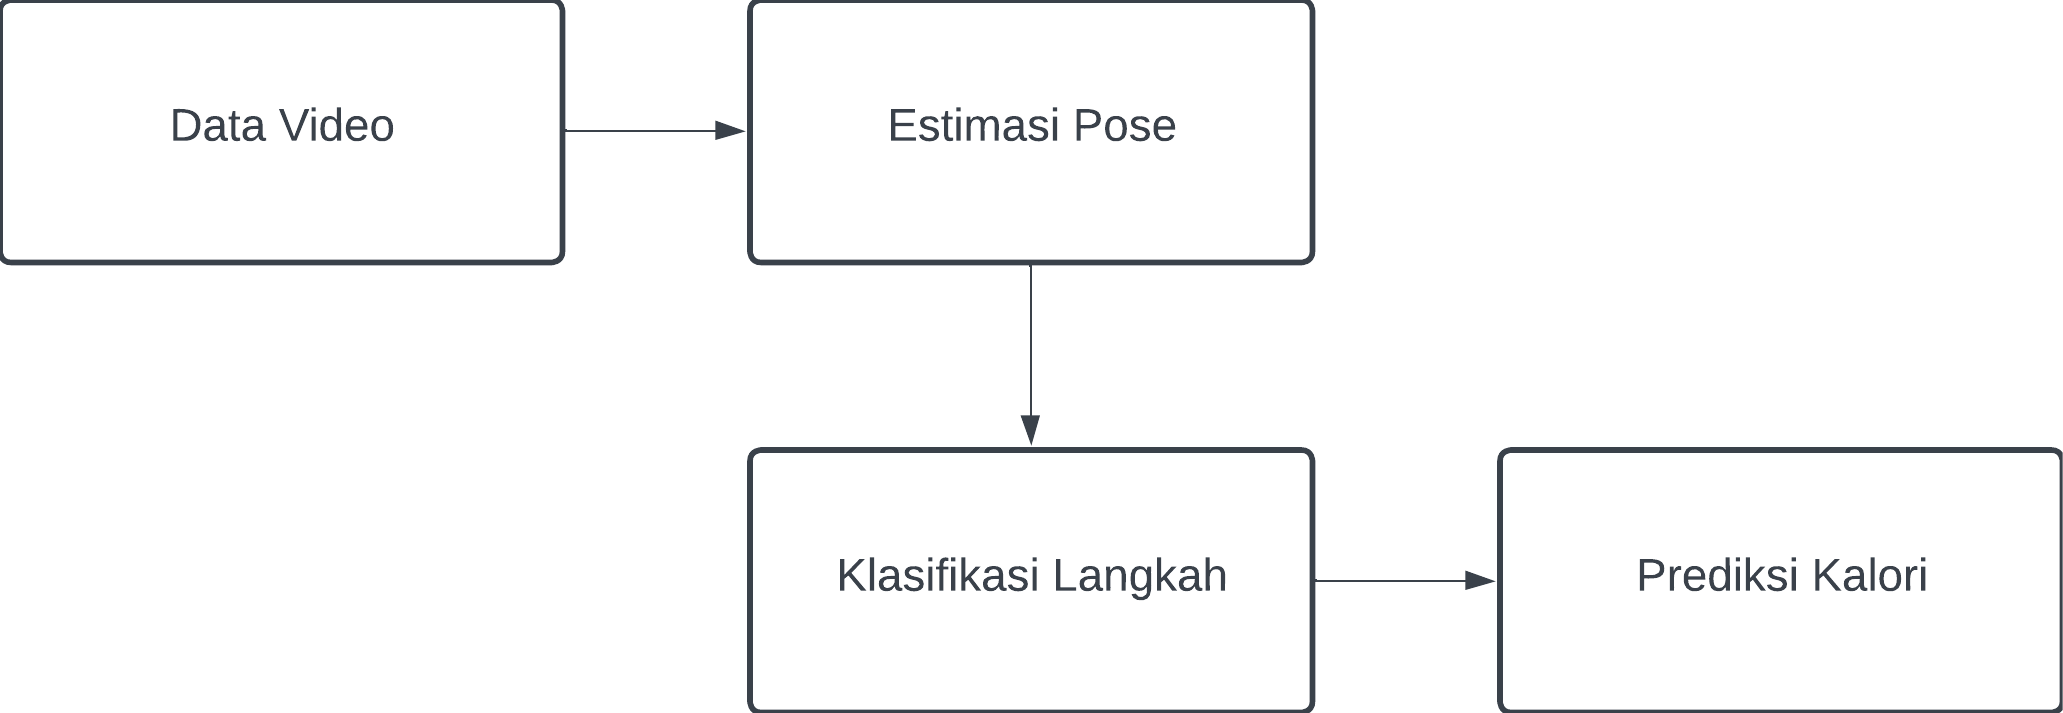
\includegraphics[width=0.4\textwidth]{gambar/blok diagram metodologi4.png}
  \caption{Bagan Umum Metodologi Sistem}
  \label{fig:BlokMetodologi}
\end{figure}

\subsection{Data Video}
\label{subsec:DataVideo}

Pada penelitian ini digunakan data berupa data video yang dilakukan pengambilan data dan diperoleh menggunakan kamera pada \emph{smartphone} atau kamera eksternal yang akan direkam dan disimpan untuk kemudian akan digunakan pada proses yang dilakukan pada perangkat komputer/laptop. Proses pengambilan data dilakukan dengan peraga melakukan aktivitas pada treadmill dengan ditampakkan secara jelas pada tampilan kamera Webcam. Setelah terdapat peraga dan tampak jelas pada tampilan maka data citra akan dilakukan pada tahap selanjutnya untuk dideteksi dan segmentasi pose seperti pada Gambar \ref{fig:DataVideo}. Variasi yang digunakan pada data video yang digunakan berdasarkan variasi kecepatan dan hasil kalori yang terbakar.

\begin{figure} [ht]
  \centering
  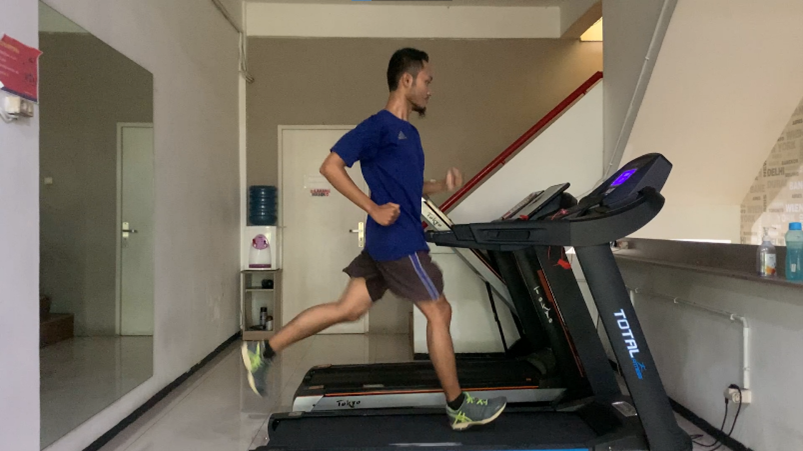
\includegraphics[width=0.4\textwidth]{gambar/pengambilan data.png}
  \caption{Proses Pengambilan Data}
  \label{fig:DataVideo}
\end{figure}

\subsection{Estimasi Pose}
\label{subsec:EstimasiPose}

Estimasi dari hasil citra untuk dapat mengetahui bentuk postur tubuh manusia menggunakan Python dengan \emph{library} OpenCV yaitu MediaPipe. Metode yang digunakan pada MediaPipe menggunakan estimasi pose untuk mendeteksi postur tubuh. Modifikasi dilakukan dengan mengambil kerangka bagian kaki dengan memberikan warna yang berbeda untuk dapat berfokus pada hasil estimasi kaki bagian kiri dan kanan. Segementasi dilakukan dengan cara peraga melakukan aktivitas \emph{jogging} pada treadmill dengan menentukan pose melangkah seperti yang terdapat pada Gambar \ref{fig:EstimasiPose}. Hasil estimasi dari model Mediapipe berupa kerangka yang menyesuaikan bentuk tubuh yang diestimasi dari data video yang dimiliki.

\begin{figure} [ht]
  \centering
  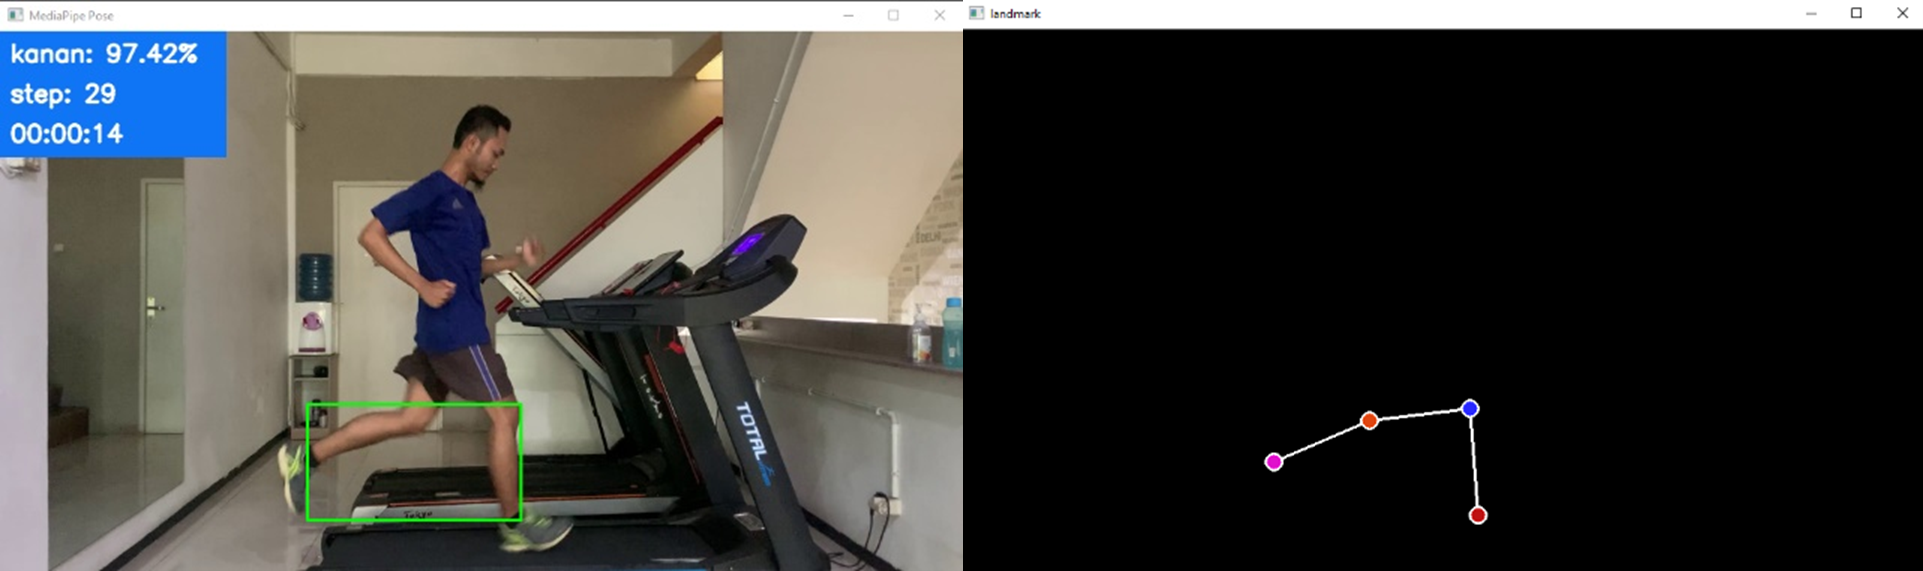
\includegraphics[width=0.4\textwidth]{gambar/deteksi pose.png}
  \caption{Deteksi Pose dengan Mediapipe}
  \label{fig:EstimasiPose}
\end{figure}

Fitur dibuat berdasarkan segmentasi pose yang telah ditentukan dan dilakukan estimasi. Semua fitur dipersiapkan sebagai kombinasi dataset yang nantinya akan digunakan pada training. Setelah menentukan fitur yang akan diekstrak, dilakukan ekstrak fitur untuk mendapatkan setiap data yang dibutuhkan dengan setiap percobaan dari kombinasi segmentasi pose. Hasil yang didapat dari ekstrak fitur berupa data set yang nantinya akan dilakukan training untuk model yang diinginkan. Dataset yang digunakan terdiri dari dua kelas dan pelabelan dari hasil deteksi dan estimasi pose, yaitu kaki “kiri” dan “kanan” seperti pada Gambar \ref{fig:DeteksiPose2}. Hasil pelabelan yang dilakukan pada hasil estimasi dan ekstrak fitur ditunjukkan pada Tabel \ref{tab:HasilAnotasi}

\begin{figure} [ht]
  \centering
  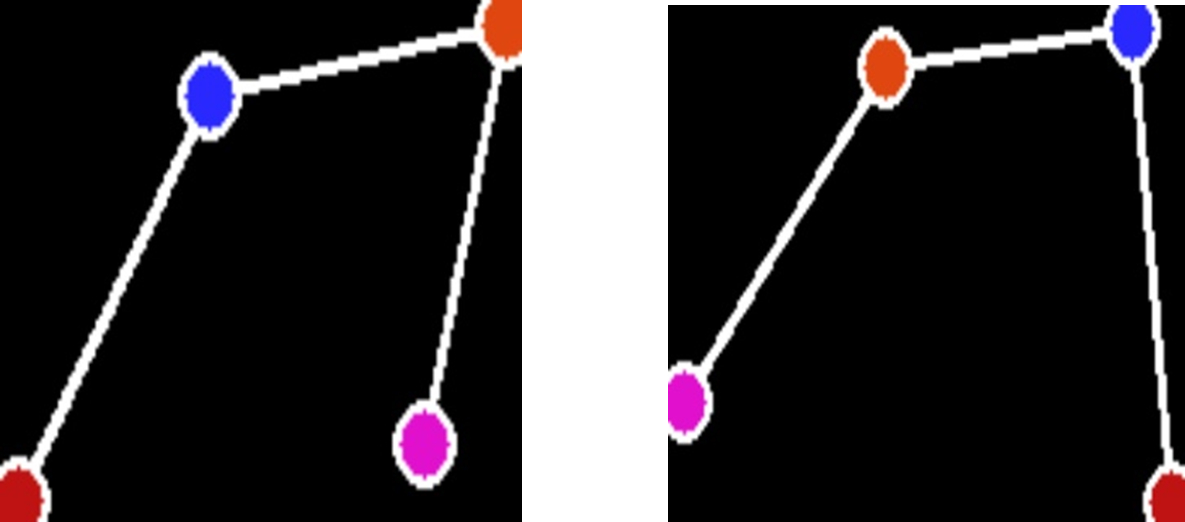
\includegraphics[width=0.4\textwidth]{gambar/deteksi pose2.png}
  \caption{Dataset Pembuatan Model}
  \label{fig:DeteksiPose2}
\end{figure}

\begin{table} [ht]
  \caption{Hasil anotasi pelabelan objek}
  \label{tab:HasilAnotasi}
  \centering
  \begin{tabular}{ll}
    \toprule
    Kelas & Jumlah Anotasi  \\
    \midrule
    Kanan       & 888    \\
    Kiri        & 843    \\
    \textbf{Total}       & \textbf{1.731}        \\
    \bottomrule
  \end{tabular}
\end{table}

\subsection{Klasifikasi Langkah}
\label{subsec:KlasifikasiLangkah}

Fitur yang telah dilakukan ekstraksi maka kemudian dilakukan training untuk memperoleh model deteksi. Model deteksi dari data set akan digunakan untuk melatih model dari sebuah algoritma pada Machine Learning. Dalam melakukan klasifikasi menggunakan Convolutional Neural Networks (CNN). Proses training ini bertujuan agar nantinya komputasi yang dilakukan dalam proses deteksi akan dapat diolah berdasarkan akuisisi data citra menjadi bentuk atau pola pemahaman yang diinginkan. Hasil training akan didapatkan model yang digunakan untuk melakukan klasifikasi atas dataset yang dimiliki yaitu terdapat dua kelas atau label untuk dapat diklasifikasikan menjadi kaki “kiri” dan “kanan”. Klasifikasi dalam menentukan aktivitas yang digunakan pada penelitian ini adalah dapat mengetahu langkah dari seseorang yang berjalan atau berlari seperti pada Gambar \ref{fig:DeteksiModel}.

\begin{figure} [ht]
  \centering
  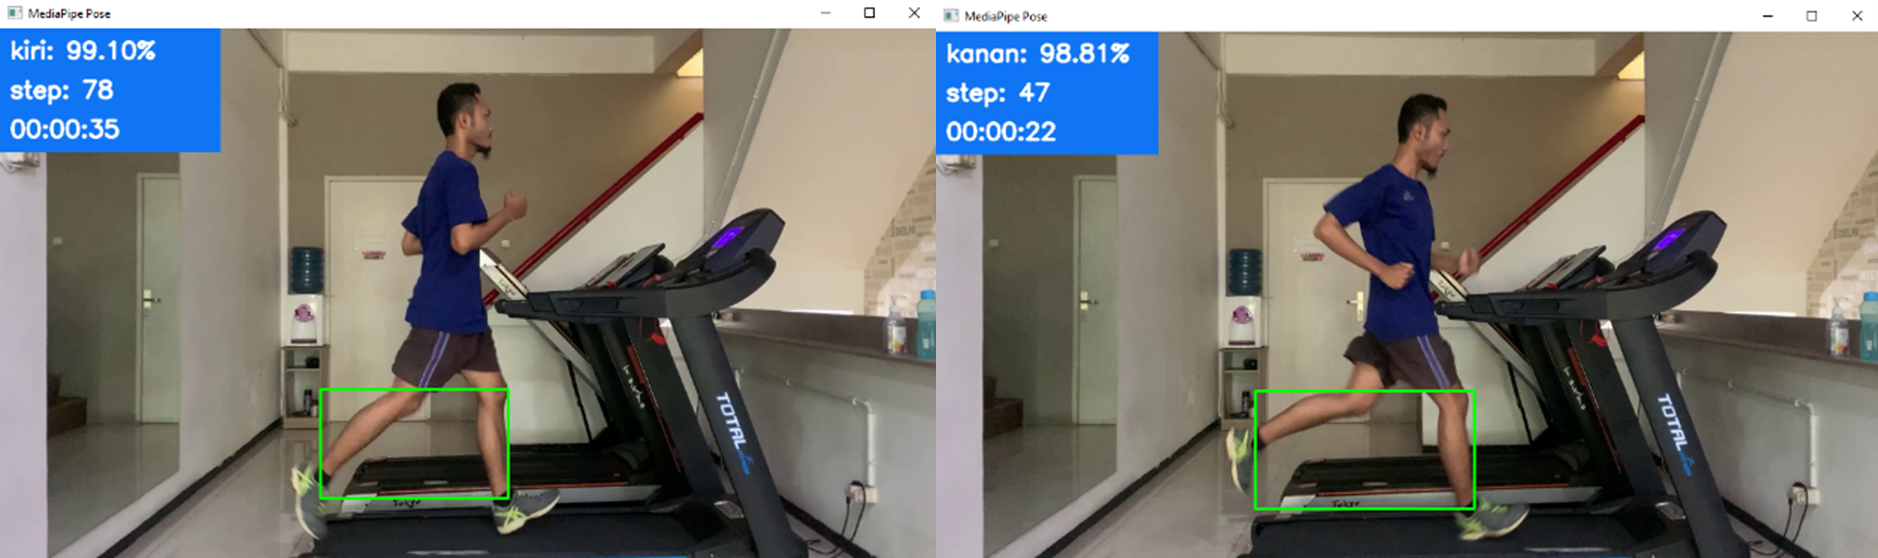
\includegraphics[width=0.4\textwidth]{gambar/deteksi.png}
  \caption{Klasifikasi pada Data Citra}
  \label{fig:DeteksiModel}
\end{figure}



Bentuk hasil klasifikasi yang dibuat adalah mendeteksi pose aktivitas dengan dapat menghitung langkah dan waktu yang ditempuh. Nilai langkah dan waktu yang ditempuh akan digunakan dalam perhitungan selanjutnya. Banyaknya jumlah langkah yang didapat saat hasil deteksi digunakan sebagai nilai variable pertama yang akan digunakan dalam penentuan perhitungan kalori. Langkah dideteksi dan dihitung seberapa banyak langkah yang dilakukan saat proses deteksi. Waktu tempuh saat proses deteksi merupakan nilai variabel kedua yang akan digunakan dalam penentuan perhitungan kalori. Waktu tempuh dimulai saat dideteksi pertama kali nilai langkah yang ditemukan hingga saat akhir langkah tidak ada penambahan kembali yang menandakan proses deteksi telah selesai. Hasil deteksi akan ditampilkan seiring dengan proses deteksi yang dilakukan pada data citra seperti pada Gambar \ref{fig:HasilDeteksi}.

\begin{figure} [ht]
  \centering
  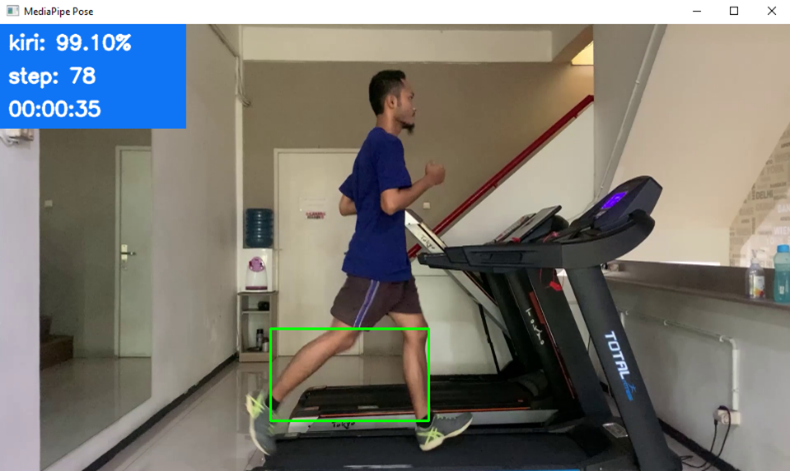
\includegraphics[width=0.4\textwidth]{gambar/hasil deteksi.png}
  \caption{Hasil Deteksi pada Citra}
  \label{fig:HasilDeteksi}
\end{figure}

\subsection{Prediksi Kalori}
\label{subsec:PrediksiKalori}

Prediksi kalori dilakukn dengan dua metode, yaitu menggunakan metode regresi linear dan menggunakan perhitungan rumus EC (Exercise Calories) berdasarkan satuan ukuran MET (Metabolic Equivalent). Kedua metode prediksi ini digunakan sebagai pembanding dalam melakukan analisa terhadap hasil yang didapatkan dari metode prediksi menggunakan metode regresi linear dengan perhitungan rumus. Data yang digunakanan dalam proses prediksi kalori diambil berdasarkan hasil klasifikasi dan hasil deteksi yang telah dilakukan sebelumnya. Hasil deteksi berupa banyaknya langkah dan waktu tempuh digunakan untuk proses prediksi kalori baik dengan metode regresi linear maupun metode perhitungan rumus.

\begin{enumerate}
  \item Regresi Linear
  
  Prediksi kalori dengan regresi linear dilakukan dengan teknik analisis untuk mengidentifikasi relasi antar dua variabel atau lebih. Pada penelitian ini varibel yang digunakan adalah hasil deteksi berupa hasil jumlah deteksi langkah dengan hasil waktu tempuh untuk nantinya akan dicari terkait relasi antara variabel tersebut untuk bisa menentukan hasil yang diinginkan yaitu prediksi kalori. Pengambilan data dilakukan dengan melakukan variasi pada alat treadmill dan didapat data waktu, keepatan dan kalori terbakar untuk dijadikan dataset model regresi. Didapatkan 1045 data sebagai dataset untuk membuat model yang akan dilakukan pengolahan data untuk dapat mendapatkan model yang diinginkan.

  Pengolahan data dilakukan dengan mengubah kecepatan menjadi jarak tempuh berdasarkan data kecepatan dan waktu. Hasil pengolahan data membuat dataset yang digunakan adalah data waktu, jarak tempuh dan kalori terbakar. Model regresi dibuat dengan menggunakan variabel independen berupa waktu dan jarak tempuh, sedangkan variabel dependen berupa kalori terbakar. Hasil proyeksi dari model regresi linear yang dibuat untuk prediksi kalori terbakar ditunjukkan pada Gambar \ref{fig:ModelRegresiKalori}.

  \begin{figure} [ht]
    \centering
    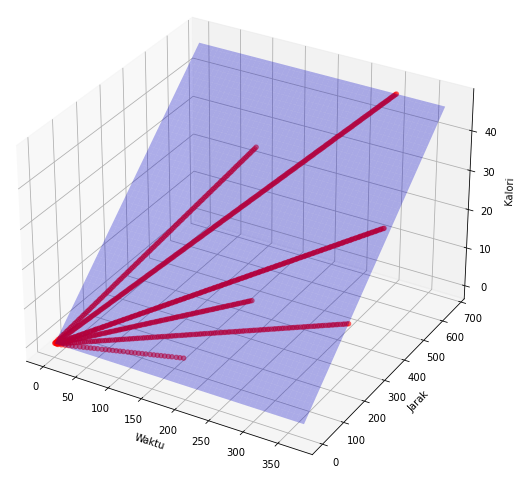
\includegraphics[width=0.4\textwidth]{gambar/model regresi kalori3.png}
    \caption{Model Regresi Linear Prediksi Kalori Terbakar}
    \label{fig:ModelRegresiKalori}
  \end{figure}

  Hasil deteksi berupa banyak langkah dan waktu tempuh diperlukan untuk melakukan pengolahan data banyak langkah menjadi jarak tempuh. Dalam menentukan jarak tempuh diperlukan untuk dapat melakukan prediksi panjang langkah untuk dikalikan dengan banyak langkah dan menghasilkan jarak tempuh. Prediksi jarak tempuh dilakukan dengan model regresi polinomial dengan dataset yang diolah menjadi data waktu, banyak langkah dan panjang langkah. Model regresi dibuat dengan menggunakan variabel independen berupa waktu dan banyak langkah, sedangkah variabel dependen berupa panjang langkah. Hasil proyeksi dari model regresi polinomial yang dibuat untuk prediksi panjang langkah ditunjukkan pada Gambar \ref{fig:ModelRegresiPanjang}.

  \begin{figure} [ht]
    \centering
    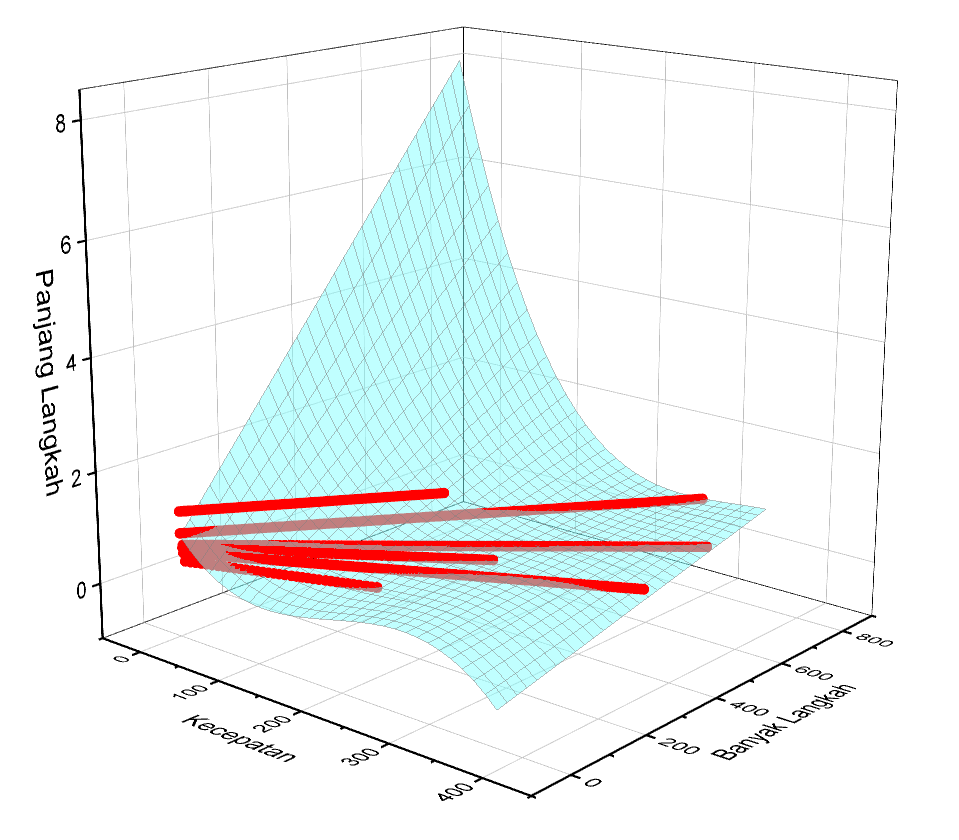
\includegraphics[width=0.4\textwidth]{gambar/model regresi panjang.png}
    \caption{Model Regresi Linear Prediksi Kalori Terbakar}
    \label{fig:ModelRegresiPanjang}
  \end{figure}

  Prediksi kalori dengan regresi dilakukan dengan mengolah hasil deteksi berupa data banyak langkah dan waktu tempuh untuk diprediksi panjang langkah dengan model regresi polinomial prediksi panjang langkah. Kemudian hasil panjang langkah dikali dengan banyak langkah untuk diketahui jarak tempuh. Hasil jarak tempuh dan waktu tempuh diprediksi untuk kalori terbakar dengan model regresi linear prediksi kalori terbakar.

  \item 
  
  Perhitungan Rumus 

  Perhitungan kalori dilakukan dengan mengacu pada nilai satuan ukuran \emph{Metabolic Equivalent} (MET). Satuan MET akan mendapat pengukuran untuk konsumsi oksigen dan pembakaran kalori. Nilai dari satuan MET dapat didefinisikan pada Persamaan \ref{eq:SatuanMET}.

  \begin{equation}
    \label{eq:SatuanMET}
    1 \mathbf{MET} = 3.5 ml O_2  / KG / min
  \end{equation}

  Berdasarkan nilai satuan ukuran MET, didapatkan suatu persamaan untuk menghitung pembakaran kalori yang didefiniskan pada Persamaan \ref{eq:RumusKalori}.

  \begin{equation}
    \label{eq:RumusKalori}
    \mathbf{Cal} = \frac{MET  * 3.5 * BB}{200} * \frac{duration}{60} calories / min
  \end{equation}

  Pada persamaan pembakaran kalori yang akan digunakan untuk melakukan perhitungan pembakaran kalori dari aktivitas yang dilakukan dibutuhkan beberapa nilai variabel untuk mendapatkah hasil total pembakaran kalori, yaitu nilai MET, nilai berat badan (BB), dan nilai waktu tempuh dalam menit.

  Setiap aktivitas memiliki nilai MET yang berbeda-beda dan telah ditentukan oleh peneliti yang telah merangkum banyak aktivitas untuk ditentukan berapa nilai MET yang dihasilkan. Pada aktivitas olahraga yang difokuskan saat ini adalah \emph{jogging} pada treadmill juga memiliki perbedaan nilai MET yang dipengaruhi oleh kecepatan. Data berkaitan dengan pengaruh kecepatan terhadap MET didapatkan yang kemudian dijadikan dataset untuk dilakukan pembuatan model regresi linear prediksi MET. Model regresi dibuat dengan menggunakan variabel independen berupa kecepatan dan variabel dependen berupa MET. Hasil proyeksi dari model regresi linear yang dibuat untuk prediksi MET ditunjukkan pada Gambar \ref{fig:ModelRegresiMET}.

  \begin{figure} [ht]
    \centering
    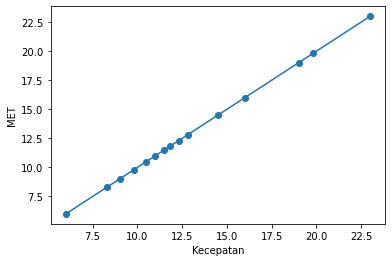
\includegraphics[width=0.4\textwidth]{gambar/model regresi met.png}
    \caption{Model Regresi Linear Prediksi MET}
    \label{fig:ModelRegresiMET}
  \end{figure}
  
  Prediksi kalori dengan perhitungan dilakukan dengan mengolah hasil deteksi berupa data banyak langkah dan waktu tempuh untuk diprediksi panjang langkah. Kemudian hasil panjang langkah dikali dengan banyak langkah untuk diketahui jarak tempuh. Hasil jarak tempuh dan waktu tempuh akan diolah untuk diketahui kecepatan tempuh. Kecepatan tempuh yang didapat dilakukan prediksi untuk MET dengan model regresi linear prediksi MET. Hasil nilai MET digunakan pada perhitungan kalori terbakar dengan data MET, waktu tempuh dan berat badan dengan nilai standar yaitu 70 kg untuk mendapatkan hasil prediksi perhitungan kalori yang terbakar.

\end{enumerate}


  % Ubah judul dan label berikut sesuai dengan yang diinginkan.
\section{Penelitian dan Pembahasan}
\label{sec:PenelitianPembahasan}

Penelitian dilakukan dengan melakukan uji dan anaisa dari sistem yang telah dibuat berdasarkan langkah pada metodologi yang telah dilaksanakan. Pengujian ini dilakukan untuk menguji kemampuan sistem yang telah dibuat dalam menjawab permasalahan yang dijadikan acuan pada penelitian ini untuk mendapatkan hasil dari tujuan yang ingin didapat. Pembahasan pengujian yang dilakukan pada penelitian ini meliputi pengujian hasil training dan validation model, pengujian hasil testing model, pengujian hasil deteksi dan pengujian prediksi.

\subsection{Pengujian Hasil Training dan Validation Model}
\label{subsec:PengujianTrainingValidation}

Pengujian pembuatan model berdasarkan hasil training dan validation dengan menggunakan dataset dengan jumlah keseluruhan yaitu 1731 sampel data. Dengan jumlah sample training sebanyak 1385 dan sampel validation sebanyak 346. Setelah dilakukan proses training dan validation terhadap dataset yang telah ditentukan oleh sampel data, didapatkan hasil pengujian akurasi dengan tingkat akurasi training sebesar 96\% dan tingkat akurasi validation sebesar 96\%. Kemudian didapatkan hasil pengujian loss pada training sebesar 0,4\% dan loss pada validation sebesar 0,4\%. Hasil pengujian ditunjukkan pada grafik nilai akurasi dan loss pada proses training dan validation seperti pada Gambar \ref{fig:GrafikTrainingValidation}

\begin{figure} [ht]
  \centering
  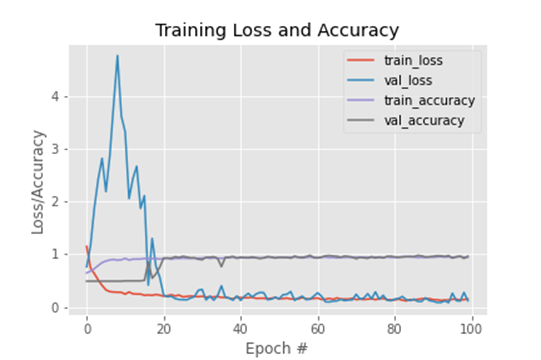
\includegraphics[width=0.4\textwidth]{gambar/hasil training dan validation.png}
  \caption{Grafik Hasil Training dan Validation Model}
  \label{fig:GrafikTrainingValidation}
\end{figure}

\subsection{Pengujian Testing Model}
\label{subsec:PengujianTesting}

Pengujian dilanjutkan dengan melakukan \emph{testing} model dengan menggunakan dataset yang sudah dimiliki dengan jumlah keseluruhan yaitu 347 sampel data. Hasil pengujian \emph{testing} model didapatkan akurasi sebesar 95\% dengan hasil deteksi benar untuk kelas kanan sebanyak 170 sampel (96\%) dan kelas kiri sebanyak 161 sampel (95\%). Pengujian ditunjukkan dengan confusion matrix pada Gambar \ref{fig:HasilTesting} dan Tabel \ref{tab:ClassificationReport} merupakan classification report dari hasil pengujian yang telah dilakukan pada pengujian \emph{testing} model penelitian ini.

\begin{figure} [ht]
  \centering
  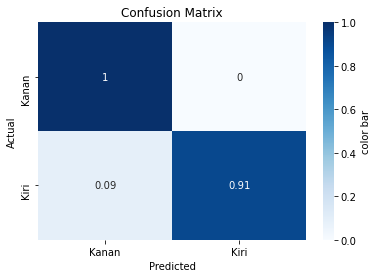
\includegraphics[width=0.4\textwidth]{gambar/cm normalized.png}
  \caption{\emph{Confusion Matrix} Hasil Pengujian Testing Model}
  \label{fig:HasilTesting}
\end{figure}

\begin{table}
  \caption{\emph{CLASSIFICATION REPORT} hasil pengujian \emph{TESTING} model}
  \label{tab:ClassificationReport}
  \centering
  \begin{tabular}{lllll}
    \toprule
     & Precision & Recall & F1-Score & Support  \\
    \midrule
    Kanan       & 0,91    & 1,00    & 0,96    & 170         \\
    Kiri        & 1,00    & 0,91    & 0,95    & 177           \\
    Accuracy    &         &         & 0,95    & 347            \\
    \bottomrule
  \end{tabular}
\end{table}

\subsection{Pengujian Hasil Deteksi}
\label{subsec:PengujianDeteksi}

Proses deteksi yang dilakukan dengan menggunakan model yang telah dibuat dilakukan pengujian dari hasil yang didapat dari hasil deteksi dengan perhitungan yang sebenarnya. Pengujian dilakukan dengan membuat data sebenarnya dengan melakukan perhitungan langkah dari akuisisi maupun data video yang digunakan dalam percobaan dan dibandingkan dengan hasil perhitungan langkah dari hasil deteksi. Tabel \ref{tab:PengujianDeteksi} menunjukkan hasil perhitungan data sebenarnya dengan data hasil deteksi terhadap langkah pada data video. Hasil yang didapat dengan melakukan pengujian hasil deteksi didapatkan hasil akurasi sebesar 99,36\% dengan hasil error sebesar 0,64\%.

\begin{table}
  \caption{Pengujian Hasil Deteksi}
  \label{tab:PengujianDeteksi}
  \centering
  \begin{tabular}{lll}
    \toprule
    Percobaan & Langkah & Deteksi Langkah  \\
    \midrule
    1   & 241   & 328    \\
    2   & 169   & 170    \\
    3   & 302   & 302    \\
    4   & 246   & 248    \\
    5   & 321   & 322    \\
    6   & 220   & 218    \\
    \bottomrule
  \end{tabular}
\end{table}


\subsection{Pengujian Prediksi}
\label{subsec:PengujianPrediksi}

Pengujian pada prediksi jumlah kalori yang terbakar dilakukan setelah melakukan pengujian pada model deteksi yang telah dilakukan. Prediksi dilakukan dengan dua metode, yaitu regresi linear dan perhitungan rumus. Dengan menggunakan dataset berupa citra video yang akan digunakan untuk melakukan prediksi kalori sebanyak 6 sampel video sehingga terdapat 6 percobaan yang dilakukan. Pada pengujian dengan regresi linear dengan melakukan proses deteksi dan menggunakan model regresi linear dalam melakukan proses prediksi kalori didapatkan beberapa data pendukung dalam hasil deteksi dan data dari hasil regresi prediksi kalori. Tabel \ref{tab:PengujianPrediksiRegresi} menunjukkan hasil deteksi dan hasil prediksi kalori dengan menggunakan regresi linear.

\begin{table}
  \caption{Pengujian Prediksi dengan Regresi Linear}
  \label{tab:PengujianPrediksiRegresi}
  \centering
  \begin{tabular}{lllll}
    \toprule
    Percobaan & Langkah & Jarak  &  Waktu & Kalori \\
    \midrule
    1   & 238   & 167,181    & 2:50    & 11,652  \\
    2   & 170   & 118,437    & 1:35    & 8,245   \\
    3   & 302   & 293,143    & 2:02    & 20,534  \\
    4   & 248   & 284,417    & 1:41    & 19,927  \\
    5   & 322   & 287,577    & 2:03    & 20,14   \\
    6   & 218   & 286,18     & 1:21    & 20,056  \\
    \bottomrule
  \end{tabular}
\end{table}

Pada pengujian dengan perhitungan rumus berdasarkan MET dilakukan dengan melalui proses deteksi dan melakukan perhitungan rumus menghasilkan beberapa data pendukung dalam perhitungan rumus dan hasil prediksi kalori yang didapat. Tabel \ref{tab:PengujianPrediksiPerhitungan} menunjukkan hasil deteksi dan hasil prediksi kalori dengan menggunakan perhitungan rumus.

\begin{table}
  \caption{Pengujian Prediksi dengan Perhitungan Rumus}
  \label{tab:PengujianPrediksiPerhitungan}
  \centering
  \begin{tabular}{lllll}
    \toprule
    Percobaan & Kecepatan & MET  &  Waktu & Kalori \\
    \midrule
    1   & 3,626   & 2,003    & 2:50    & 6,788   \\
    2   & 5,016   & 2,733    & 1:35    & 4.744   \\
    3   & 8,943   & 9,323    & 2:02    & 22.462  \\
    4   & 10,893  & 10,721   & 1:41    & 20.575  \\
    5   & 8,151   & 8,533    & 2:03    & 22.126  \\
    6   & 13,041  & 11,985   & 1:21    & 19.331  \\
    \bottomrule
  \end{tabular}
\end{table}

Hasil yang diperoleh melalui model yang telah dibuat untuk deteksi dan melakukan prediksi sesuai metode yang dilakukan didapatkan hasil akumulasi kalori dengan prediksi regresi sebesar 93,61\% dengan akumulasi error sebesar 6,39\%. Kemudian prediksi dengan perhitungan rumus didapatkan hasil akumulasi akurasi kalori sebesar 81,03\% dengan akumulasi error sebesar 18,97\%. Tabel \ref{tab:PengujianPrediksi} merupakan hasil perbandingan antara dataset percobaan dengan nilai kalori pembanding dataset dengan proses prediksi.

\begin{table}
  \caption{Pengujian Hasil Prediksi Kalori}
  \label{tab:PengujianPrediksi}
  \centering
  \begin{tabular}{lllll}
    \toprule
    Percobaan & Kecepatan & Kalori  &  Regresi & Perhitungan \\
    \midrule
    1   & 3     & 10    & 11,652    & 6,788   \\
    2   & 6     & 10    & 8,245     & 4,744   \\
    3   & 9     & 20    & 20,534    & 22,462   \\
    4   & 12    & 20    & 19,927    & 20,575   \\
    5   & 8     & 20    & 20,14     & 22,126   \\
    6   & 12    & 20    & 20,056    & 19,331   \\
    \bottomrule
  \end{tabular}
\end{table}

  % Ubah judul dan label berikut sesuai dengan yang diinginkan.
\section{Kesimpulan}
\label{sec:kesimpulan}

Simpulan


  % Menampilkan daftar pustaka dengan format IEEE
  \begin{thebibliography}{}
    \bibitem{ano05}
      World Health Organization. (2022). Noncommunicable diseases: progress monitor 2022. World Health Organization. https://apps.who.int/iris/handle/10665/353048. License: CC BY-NC-SA 3.0 IGO
   \bibitem{ano05}
      Blüher, M. (2019). Obesity: global epidemiology and pathogenesis. Nature Reviews Endocrinology. doi:10.1038/s41574-019-0176-8
   \bibitem{ano05}
      World Health Organization. (2022). Global status report on physical activity 2022. World Health Organization. https://apps.who.int/iris/handle/10665/363607. License: CC BY-NC-SA 3.0 IGO
   \bibitem{ano05}
      Caballero, Y., Ando, T. J., Nakae, S., Usui, C., Aoyama, T., Nakanishi, M., … Tanaka, S. (2019). Simple Prediction of Metabolic Equivalents of Daily Activities Using Heart Rate Monitor without Calibration of Individuals. International Journal of Environmental Research and Public Health, 17(1), 216. doi:10.3390/ijerph17010216
   \bibitem{ano05}
      Safaei, M., Sundararajan, E. A., Driss, M., Boulila, W., \& Shapi’i, A. (2021). A systematic literature review on obesity: Understanding the causes \& consequences of obesity and reviewing various machine learning approaches used to predict obesity. Computers in Biology and Medicine, 136, 104754. doi:10.1016/j.compbiomed.2021.104754 
   \bibitem{ano05}
      Bohlen, A., Boll, M., Schwarzer, M., \& Groneberg, D. A. (2014). Body-Mass-Index. Zentralblatt Für Arbeitsmedizin, Arbeitsschutz Und Ergonomie, 64(6), 415–429. doi:10.1007/s40664-014-0074-9
   \bibitem{ano05}
      Lobstein, T. et al., 2023. World Obesity Atlas 2023, World Obesity Federation. United Kingdom.
   \bibitem{ano05}
      Kevin D Hall and others, The energy balance model of obesity: beyond calories in, calories out, The American Journal of Clinical Nutrition, Volume 115, Issue 5, May 2022, Pages 1243–1254, https://doi.org/10.1093/ajcn/nqac031
   \bibitem{ano05}
      Anderson, E., \& Durstine, J. L. (2019). Physical Activity, Exercise, and Chronic Diseases: A Brief Review. Sports Medicine and Health Science. doi:10.1016/j.smhs.2019.08.006
   \bibitem{ano05}
      Erkkola, R. U., Vasankari, T., \& Erkola, A. (2020). Opinion paper: Exercise for healthy aging. Maturitas. doi:10.1016/j.maturitas.2020.10.012 
   \bibitem{ano05}
      Pojednic, R.; D'Arpino, E.; Halliday, I.; Bantham, A. The Benefits of Physical Activity for People with Obesity, Independent of Weight Loss: A Systematic Review. Int. J. Environ. Res. Public Health 2022, 19, 4981. https://doi.org/10.3390/ijerph19094981
   \bibitem{ano05}
      Marquez, D. X., Aguiñaga, S., Vásquez, P. M., Conroy, D. E., Erickson, K. I., Hillman, C., … Powell, K. E. (2020). A systematic review of physical activity and quality of life and well-being. Translational Behavioral Medicine, 10(5), 1098–1109. doi:10.1093/tbm/ibz198
   \bibitem{ano05}
      Gaesser, Glenn \& Angadi, Siddhartha. (2021). Obesity treatment: Weight loss versus increasing fitness and physical activity for reducing health risks. iScience. 24. 10.1016/j.isci.2021.102995.
   \bibitem{ano05}
      Nurhayati, Faridha \& Wahjuni, Endang \& Andrijanto, Dony \& Febriyanti, Irma \& Kaharina, Arifah. (2020). Quality of Life and Level of Physical Activity in Sports Education Students During the COVID-19 Pandemic. 10.2991/assehr.k.201201.196.
    \bibitem{oe04}
      Theunissen, K., Van Hooren, B., Plasqui, G., \& Meijer, K. (2022). Self-paced and fixed speed treadmill walking yield similar energetics and biomechanics across different speeds. Gait \& posture, 92, 2–7. https://doi.org/10.1016/j.gaitpost.2021.11.005
    \bibitem{oe04}
      Miller, J. R., Van Hooren, B., Bishop, C., Buckley, J. D., Willy, R. W., \& Fuller, J. T. (2019). A Systematic Review and Meta-Analysis of Crossover Studies Comparing Physiological, Perceptual and Performance Measures Between Treadmill and Overground Running. Sports Medicine, 49(5), 763–782. doi:10.1007/s40279-019-01087-9 
    \bibitem{oe04}
      Wiens, C., Denton, W., Schieber, M. N., Hartley, R., Marmelat, V., Myers, S. A., \& Yentes, J. M. (2019). Walking speed and spatiotemporal step mean measures are reliable during feedback-controlled treadmill walking; however, spatiotemporal step variability is not reliable. Journal of Biomechanics. doi:10.1016/j.jbiomech.2018.11.051 
    \bibitem{oe04}
      Ibala, Eunice \& Coupaud, Sylvie \& Kerr, Andy. (2019). Comparison of the Muscle Pattern Variability During Treadmill Walking (Fixed and Self-Pace) and Over Ground Walking of Able-Bodied Adults Journal of Annals of Bioengineering Citation. Journal of Annals of Bioengineering. 1. 1-11. 10.33513/BIOE/1901-04. 
    \bibitem{oe04}
      Nouriani, A., McGovern, R., \& Rajamani, R. (2023). Activity Recognition Using A Combination of High Gain Observer and Deep Learning Computer Vision Algorithms. Intelligent Systems with Applications. Volume 18, ISSN 2667-3053. doi: 10.1016/j.iswa.2023.200213.
    \bibitem{oe04}
      Chai, J., Zeng, H., Li, A., \& Ngai, E. W. T. (2021). Deep learning in computer vision: A critical review of emerging techniques and application scenarios. Machine Learning with Applications, 6, 100134. doi:10.1016/j.mlwa.2021.100134 
    \bibitem{oe04}
      Hou, C. (2020). A study on IMU-Based Human Activity Recognition Using Deep Learning and Traditional Machine Learning. 2020 5th International Conference on Computer and Communication Systems (ICCCS). doi:10.1109/icccs49078.2020.9118506
    \bibitem{oe04}
      Ramanujam, E., Perumal, T., \& Padmavathi, S. (2021). Human Activity Recognition With Smartphone and Wearable Sensors Using Deep Learning Techniques: A Review. IEEE Sensors Journal, 21(12), 13029–13040. doi:10.1109/jsen.2021.3069927 
  

    \end{thebibliography}

  % Menyeimbangkan bagian akhir di kedua kolom
  \balance

\end{document}
